\documentclass[
	% -- opções da classe memoir --
	12pt,				% tamanho da fonte
	%openright,			% capítulos começam em pág ímpar (insere página vazia caso preciso)
	oneside,			% para impressão em recto e verso. Oposto a oneside
	a4paper,			% tamanho do papel. 
	% -- opções da classe abntex2 --
	%chapter=TITLE,		% títulos de capítulos convertidos em letras maiúsculas
	%section=TITLE,		% títulos de seções convertidos em letras maiúsculas
	%subsection=TITLE,	% títulos de subseções convertidos em letras maiúsculas
	%subsubsection=TITLE,% títulos de subsubseções convertidos em letras maiúsculas
	% -- opções do pacote babel --
	english,			% idioma adicional para hifenização
	french,				% idioma adicional para hifenização
	spanish,			% idioma adicional para hifenização
	brazil,				% o último idioma é o principal do documento
	]{abntex2}


% ---
% PACOTES
% ---

% ---
% Pacotes fundamentais 
% ---
\usepackage{pslatex}			% Usa a fonte Latin Modern
\usepackage[T1]{fontenc}		% Selecao de codigos de fonte.
\usepackage[utf8]{inputenc}		% Codificacao do documento (conversão automática dos acentos)
\usepackage{indentfirst}		% Indenta o primeiro parágrafo de cada seção.
\usepackage{color}				% Controle das cores
\usepackage{graphicx}			% Inclusão de gráficos
\usepackage{microtype} 			% para melhorias de justificação
\usepackage{transparent}
\usepackage{eso-pic}
\usepackage{float}
\usepackage{array}
\usepackage{epstopdf}
\usepackage{url}
% ---

% ---
% Pacotes adicionais, usados no anexo do modelo de folha de identificação
% ---
\usepackage{multicol}
\usepackage{multirow}
% ---
	
% ---
% Pacotes adicionais, usados apenas no âmbito do Modelo Canônico do abnteX2
% ---
%\usepackage{lipsum}				% para geração de dummy text
% ---

% ---
% Pacotes de citações
% ---
%\usepackage[brazilian,hyperpageref]{backref}	 % Paginas com as citações na bibl
%\usepackage[alf]{abntex2cite}	% Citações padrão ABNT

% --- 
% CONFIGURAÇÕES DE PACOTES
% --- 

% ---
% Configurações do pacote backref
% Usado sem a opção hyperpageref de backref
%\renewcommand{\backrefpagesname}{Citado na(s) página(s):~}
% Texto padrão antes do número das páginas
%\renewcommand{\backref}{}
% Define os textos da citação
%\renewcommand*{\backrefalt}[4]{
%	\ifcase #1 %
%		Nenhuma citação no texto.%
%	\or
%		Citado na página #2.%
%	\else
%		Citado #1 vezes nas páginas #2.%
%	\fi}%
% ---

% ---
% Informações de dados para CAPA e FOLHA DE ROSTO
% ---
\titulo{Estatística e Probabilidade\\Trabalho sobre Apresentação de Dados\\ Parte 1 - Teórica}
\autor{Profª Drª Mara Lúcia Martins Lopes\\Caio da Silva Pereira\\Gabriel Rodrigues Munhoz\\Heitor Martins da Silva\\Leandro Suzuki Barboza dos Santos\\Rafael Gomes de Oliveira\\Thiago Rissetti Roquetto}
\local{Ilha Solteira, São Paulo}
\data{Setembro de 2017}
\instituicao{%
  Universidade Estadual Paulista  - Unesp
  \par
  Faculdade de Engenharia de Ilha Solteira  - FEIS}
\tipotrabalho{Trabalho científico}
% O preambulo deve conter o tipo do trabalho, o objetivo, 
% o nome da instituição e a área de concentração 
\preambulo{"Estatística é método, ciência e arte."}
% ---

% ---
% Configurações de aparência do PDF final

% alterando o aspecto da cor azul
\definecolor{blue}{RGB}{41,5,195}

% informações do PDF
\makeatletter
\hypersetup{
     	%pagebackref=true,
		pdftitle={\@title}, 
		pdfauthor={\@author},
    	pdfsubject={\imprimirpreambulo},
	    pdfcreator={LaTeX with abnTeX2},
		pdfkeywords={abnt}{latex}{abntex}{abntex2}{relatório técnico}, 
		colorlinks=true,       		% false: boxed links; true: colored links
    	linkcolor=blue,          	% color of internal links
    	citecolor=blue,        		% color of links to bibliography
    	filecolor=magenta,      		% color of file links
		urlcolor=blue,
		bookmarksdepth=4
}
\makeatother
% --- 

% --- 
% Espaçamentos entre linhas e parágrafos 
% --- 

% O tamanho do parágrafo é dado por:
\setlength{\parindent}{1.3cm}

% Controle do espaçamento entre um parágrafo e outro:
\setlength{\parskip}{0.2cm}  % tente também \onelineskip

% ---
% compila o indice
% ---
\makeindex
% ---
\usepackage{fancyhdr}
\fancyhead{}
\fancyfoot{}
\lhead{Trabalho sobre Ajustagem Mecânica}
\rhead{\thepage}

\AddToShipoutPicture{

\put(0,0){

\parbox[b][\paperheight]{\paperwidth}{%

\vfill

\centering

{\transparent{0.1}\includegraphics[scale=2]{../../../Imagens/SA03x.jpg}  }%

\vfill}}}
% ----
% Início do documento
% ----
\begin{document}

\begin{minipage}[c][1.5cm][c]{3cm} % a primeira minipágina tem uma altura de 1.5cm e uma largura de 3cm.

\includegraphics[scale=0.6]{../../../Imagens/barraunesp-assvisual.png} 

\end{minipage}

% Seleciona o idioma do documento (conforme pacotes do babel)
%\selectlanguage{english}
\selectlanguage{brazil}

% Retira espaço extra obsoleto entre as frases.
\frenchspacing 

% ----------------------------------------------------------
% ELEMENTOS PRÉ-TEXTUAIS
% ----------------------------------------------------------
%\pretextual

% ---
% Capa
% ---
\imprimircapa
% ---

% ---
% Folha de rosto
% (o * indica que haverá a ficha bibliográfica)
% ---
\imprimirfolhaderosto*

% ---
% inserir o sumario
% ---
\pdfbookmark[0]{\contentsname}{toc}
\tableofcontents*
\newpage

\section[Introdução]{Introdução}
\pagestyle{fancy}

Estatística pode ser pensada como a ciência de aprendizagem a partir de dados. Logo, temos que apresentar esses dados e organizá-los para que o nosso estudo acerca deles se simplifique e seja correto. Podemos dividir a estatística em dois ramos, o primeiro sendo o descritivo que é composto por toda a parte de coleta, organização, descrição e cálculo dos dados; e a segunda que é o ramo indutivo que é formado pela análise e interpretação, associados a uma margem de incerteza. \cite{wiki}

Existem diferentes tipos de variáveis e para que tal estudo sobre elas ocorra de forma ordenada há diferentes tipos de distribuição de frequência e gráficos para simplificar a visualização de cada tipo.

Primeiramente iremos diferenciar os tipos de variáveis e em seguida expor todos os principais modelos de tabelas e gráficos. Tudo isso junto compõe os diferentes tipos de apresentações de dados.

\newpage
\section[Variáveis]{Variáveis}

Uma variável é aquilo que se deseja observar para tirar algum tipo de conclusão. Os dados de uma certa pesquisa são compostos por variáveis. Essas, podem ser divididas em: 

\begin{center}
•	Variáveis Qualitativas;\\
•	Variáveis Quantitativas;\\

\end{center}
\subsection{Variáveis Qualitativas}

As variáveis qualitativas não podem ser expressas numericamente, pois relacionam
situações como cor da pele, cor dos olhos, marca de refrigerante, marca de automóvel entre
outras. Podem ser divididas em ordinais e nominais.\cite{variaveis}

\subsubsection{Variáveis Qualitativas Nominais}

Não estão relacionadas a ordem, elas são identificadas apenas por nomes, por
exemplo, as cores: Vermelho, amarelo, preto, azul, rosa, verde. Além das cores temos as
marcas de carros, nome de bebidas, local de nascimento.\cite{variaveis5}

Um exemplo mais concreto se vê na observação de ursos, separando-os por sexo, não
há uma ordem natural em suas categorias, a ordem na linha das tabelas pode ser qualquer
uma, nesse caso se dá por:

\begin{center}
\begin{table}[H]
\caption{Distribuição de Dados Qualitativos Nominais}
\begin{center}
\begin{tabular}{c|c|c}

\hline
Sexo & Frequência Absoluta & Frequência Relativa$(\%)$ \\ 
\hline
Feminino & 35 & 36,1 \\
\hline
Masculino & 62 & 63,9 \\
\hline
Total & 97 & 100,0 \\

\end{tabular}
\end{center}
\legend{Fonte: Elaborado pelo autor}
\end{table}
\end{center}

\subsubsection{Variáveis Qualitativas Ordinais}

Nem sempre são numéricas, mas obedecem a uma relação de ordem, por exemplo,
conceitos como ótimo, bom, regular e ruim, classe social, grau de instrução.\cite{variaveis5}

No caso da observação dos ursos, a distribuição de frequência dos ursos segundo o
mês de observação representa uma variável qualitativa ordinal, segue a tabela:

\begin{center}
\begin{table}[htbp]
\caption{Exemplo de variável qualitativa ordinal: Distribuição de frequência dos 97 ursos
segundo mês de observação.}
\begin{center}
\begin{tabular}{>{\centering\arraybackslash}m{2cm}|>{\centering\arraybackslash}m{2cm}|>{\centering\arraybackslash}m{2cm}|>{\centering\arraybackslash}m{2cm}|>{\centering\arraybackslash}m{2cm}}

\hline
Mês de Observação & Frequência Absoluta & Frequência Relativa$(\%)$ & Frequência Absoluta Acumulada & Frequência Relativa Acumulada \\ 
\hline
Abril & 8 & 8,3 & 8 & 8,3 \\
\hline
Maio & 6 & 6,2 & 14 & 14,5 \\
\hline
Junho & 6 & 6,2 & 20 & 20,7 \\
\hline
Julho & 11 & 11,3 & 31 & 32,0 \\
\hline
Agosto & 23 & 23,7 & 54 & 55,7 \\
\hline
Setembro & 20 & 20,6 & 74 & 76,3 \\
\hline
Outubro & 14 & 14,4 & 88 & 90,7 \\
\hline
Novembro & 9 & 9,3 & 97 & 100,0 \\
\hline
Total & 97 & 100,0 & -- & -- \\

\end{tabular}
\end{center}
\legend{Fonte: www.Google.com.br}
\end{table}
\end{center}

\subsection{Variáveis Quantitativas}

As variáveis quantitativas são as características que podem ser medidas em uma escala quantitativa, ou seja, apresentam valores numéricos que fazem sentido. Podem ser contínuas ou discretas.

\subsubsection{Variáveis Discretas}

São características mensuráveis que podem assumir apenas um número finito ou infinito contável de valores e, assim, somente fazem sentido valores inteiros. Geralmente são o resultado de contagens. Variáveis discretas são como: número de filhos, número de bactérias por litro de leite, números de garrafas quebradas em uma fabrica e assim por diante. \cite{variaveis}

\subsubsection{Variáveis Contínuas}

Essas variáveis, diferentemente das discretas, podem possuir valores fracionados, pois, são organizados em intervalos e com isso podem possuir quaisquer número entre os limites inferior e superior. Usualmente devem ser medidas através de algum instrumento. Exemplos: peso (balança), altura (régua), tempo (relógio), pressão arterial, idade. \cite{variaveis}

\newpage
\section[Distribuição de Frequência]{Distribuição de Frequência}

A distribuição de frequência é um arranjo de valores, organizando os dados para que assim possam ser melhor utilizados. Primeiramente possuímos os dados brutos que foram coletados de uma certa pesquisa, para organizá-los precisamos colocá-los em rol (em ordem crescente) e em seguida transferí-los para uma tabela de frequência. As tabelas de freqüência servem de base para as representações gráficas.

Existem dois tipos de tabelas: 

\begin{center}
•	Tabela para Variáveis Qualitativas;\\
•	Tabela para Variáveis Quantitativas;\\

\end{center}

\subsection{Tabela para Variáveis Qualitativas}

É organizada na maioria das vezes em 3 colunas, sendo a primeira preenchida pelos dados qualitativos, a segunda a frequência absoluta e por último a frequência relativa. \cite{dados}

\textbf{Exemplo:}

\begin{center}
\begin{table}[H]
\caption{Cor dos olhos de uma certa amostra de população}
\begin{center}
\begin{tabular}{c|c|c}

\hline
Categoria & Frequência Absoluta & Frequência Relativa$(\%)$ \\ 
\hline
Castanhos & 10 & 0,50 \\
\hline
Pretos & 7 & 0,35 \\
\hline
Azuis & 2 & 0,10 \\
\hline
Verdes & 1 & 0,05 \\
\hline
Total & 20 & 1,00 \\

\end{tabular}
\end{center}
\legend{Fonte: www.Google.com.br}
\end{table}
\end{center}

\subsection{Tabela para Variáveis Quantitativos}

Esse tipo de tabela é subdividido em dois tipos: de ordem discreta e de ordem contínua. Ambos possuem frequência absoluta, relativa e a acumulada. O que difere uma da outra é o modo como estão os dados, se são pontuais ou se estão em intervalos.

\subsubsection{Tabela para Dados de tipo Quantitativo Discreto}

Um exemplo de tabela para dados discretos: Número de irmãos em 20 alunos de uma turma.

\begin{center}
\begin{table}[H]
\caption{Tabela de Frequência do Número de Irmãos}
\begin{center}
\begin{tabular}{>{\centering\arraybackslash}m{2cm}|>{\centering\arraybackslash}m{2cm}|>{\centering\arraybackslash}m{2cm}|>{\centering\arraybackslash}m{2cm}|>{\centering\arraybackslash}m{2cm}}

\hline
Classe & Frequência Absoluta & Frequência Relativa$(\%)$ & Frequência Absoluta Acumulada & Frequência Relativa Acumulada \\ 
\hline
0 & 5 & 25 & 5 & 25 \\
\hline
1 & 8 & 40 & 13 & 65 \\
\hline
2 & 5 & 25 & 18 & 90 \\
\hline
3 & 2 & 10 & 20 & 100 \\
\hline
Total & 20 & 100 &  &  \\


\end{tabular}
\end{center}
\legend{Fonte: www.Google.com.br}
\end{table}
\end{center}

Convém salientar que as colunas referentes às frequências acumuladas só fazem sentido em tabelas de frequências onde a variável em estudo se possa ordenar ( no exemplo da tabela de frequências para dados de tipo qualitativo, apresentado anteriormente, não tem sentido considerar as frequências acumuladas).\cite{dados}

\subsubsection{Tabela para Dados de tipo Quantitativo Contínuo}

Se os dados são de natureza quantitativa contínua, consideram-se classes na forma de intervalos. Sempre que possível estes intervalos devem ter a mesma amplitude.

\textbf{Exemplo:}

Considerando a seguinte amostra que resultou de observar a variável Altura em 30 alunos de uma turma.

\begin{center}
\begin{table}[htbp]
\caption{Tabela de Frequência da Altura dos Alunos}
\begin{center}
\begin{tabular}{>{\centering\arraybackslash}m{2cm}|>{\centering\arraybackslash}m{2cm}|>{\centering\arraybackslash}m{2cm}|>{\centering\arraybackslash}m{2cm}|>{\centering\arraybackslash}m{2cm}}

\hline
Classes & Frequência Absoluta & Frequência Relativa$(\%)$ & Frequência Absoluta Acumulada & Frequência Relativa Acumulada \\ 
\hline
131$\vdash$ 141 & 2 & 7 & 2 & 7 \\
\hline
141$\vdash$ 151 & 6 & 20 & 8 & 27 \\
\hline
151$\vdash$ 161 & 7 & 23 & 15 & 50 \\
\hline
161$\vdash$ 171 & 9 & 30 & 24 & 80 \\
\hline
171$\vdash$ 181 & 6 & 20 & 30 & 100 \\
\hline
Total & 30 & 100 &  &  \\


\end{tabular}
\end{center}
\legend{Fonte: www.Google.com.br}
\end{table}
\end{center}

\newpage
\section[Gráficos]{Gráficos}

Gráfico é uma composição de barras, colunas ou qualquer elemento que consiga expressar a valor dos dados de forma visual. Assim, podemos dizer que os gráficos foram criados para que possamos compreender o que se passa com um certo experimento ou pesquisa apenas olhando para os diferentes tamanhos dos elementos ou as linhas que o complementam. Esse estilo de apresentação de dados pode ser dividido em:

\begin{center}
•	Gráficos para Variáveis Qualitativas;\\
•	Gráficos para Variáveis Quantitativas;\\

\end{center}

\subsection{Gráficos para Variáveis Qualitativas}

A representação de gráficos de variáveis qualitativas possui várias formas,
onde vários são apenas variações do mesmo princípio. Esta representação é feita basicamente na forma de gráficos de barras ou
colunas, ou gráficos de setores $(pizza)$, com suas diversas variações.\cite{variaveis1}

Podem, também, ser utilizados gráficos pictóricos, que, na são como variações
dos gráficos de barras. Todos os gráficos também podem ser usados para gerar gráficos de variáveis
quantitativas discretas.

\subsubsection{Gráfico de Barras}

Este tipo de gráfico possui como vantagem a sua forma simples, que permite visualizar as diferenças entre os dados com maior facilidade e rapidez. Tem a finalidade de comparar grandezas por meio de retângulos de igual largura e alturas proporcionais às respectivas grandezas.

Neste tipo de gráfico, cada barra representa a intensidade ou frequência de uma categoria ou atributo. Os espaços existentes entre as barras devem ser iguais.É preferível a este quando as legendas das categorias forem mais curtas, por maior facilidade de posicionamento e formatação.\cite{variaveis1}

Na área geográfica este gráfico é muito utilizado, seja para representar fenômenos geográficos ou as diferentes etnias de um determinado local. \\


\textbf{Gráfico de Barras Horizontais:}

Exemplo: Causas mais frequentes de intoxicação e envenenamento em crianças de 1 a 5, anos em valores absolutos

\begin{figure}[H]
\begin{center}

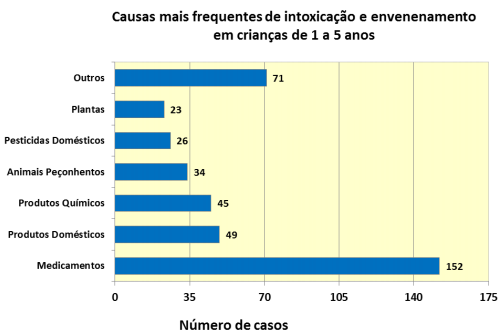
\includegraphics[scale=0.9]{grafico.jpg}  

\legend{Fonte: www.Google.com.br}
\end{center}
\end{figure}

\textbf{Gráfico de Colunas:}

Este tipo de gráfico possui a mesma finalidade do gráfico de barras, entretanto, este neste as barras são posicionadas na vertical, de maneira a formar colunas.

\textbf{Exemplo:} 

Causas mais frequentes de intoxicação e envenenamento em crianças de 1 a 5, anos em valores absolutos.

\begin{figure}[H]
\begin{center}

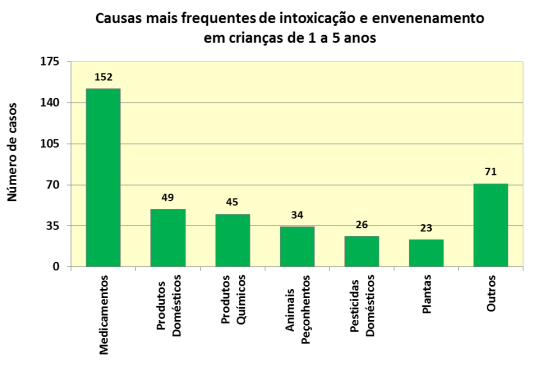
\includegraphics[scale=0.8]{grafico2.jpg}  

\legend{Fonte: www.Google.com.br}
\end{center}
\end{figure}

\subsubsection{Gráfico de Pizza}

Para construir este gráfico tem-se que encontrar a frequência relativa a princípio de cada setor a ser analisado.\cite{variaveis3} Para maior precisão nesse gráfico o ângulo central deve ser calculado, para que assim a disposição de cada categoria não fique de forma confusa, para encontrar tal ângulo multiplica-se a frequência relativa $(\%)$ por $360^{\circ}$ assim encontrasse o ângulo exato que deve ser desenhado.

\textbf{Gráfico de Setores:}

Este tipo de gráfico é a representação dos dados estatísticos em um círculo através de setores. De modo que as áreas são proporcionais aos valores da série. Utilizado principalmente para verificação de percentuais de cada valor da série com o total.\cite{variaveis4}

\begin{figure}[H]
\begin{center}

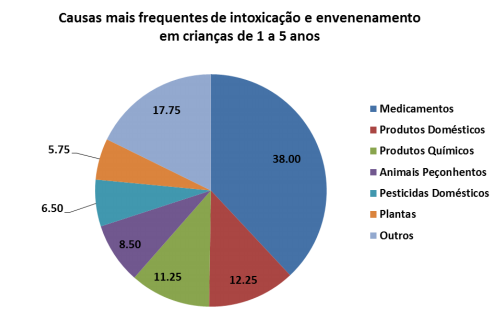
\includegraphics[scale=0.75]{grafico3.jpg}  

\legend{Fonte: www.Google.com.br}
\end{center}
\end{figure}

\textbf{Gráfico de Rosca:}

Uma das variações do gráfico de pizza é o gráfico de rosca.

\begin{figure}[H]
\begin{center}

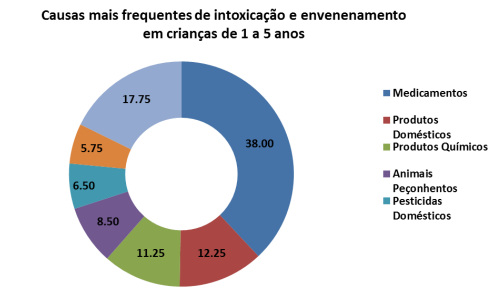
\includegraphics[scale=0.75]{grafico4.jpg}  

\legend{Fonte: www.Google.com.br}
\end{center}
\end{figure}

\subsection{Gráficos para Variáveis Quantitativas}

Os gráficos para variáveis quantitativas representam as tabelas de distribuição contínua e discreta de forma mais visual. Eles são os mais utilizados quando estamos trabalhando com dados estatísticos, pois o histograma e o boxplot expressam os dados de forma organizada e que facilita nosso entendimento.\cite{wiki}

\subsubsection{Histograma}

O gráfico de histograma remete a dados quantitativos contínuos. Esse tipo de gráfico é
utilizado para nos mostrar a frequência dos dados. Existem alguns subtipos desse gráfico
e um deles é relacionado com a frequência relativa, fazendo com que a área de cada
retângulo no gráfico represente essa frequência, assim a área total é igual a 1. Quando os
intervalos possuem mesma amplitude sua altura é definida pela frequência de cada dado.\cite{histograma}

Outro subtipo desse gráfico é o chamado usual, quando os dados representam a
frequência absoluta. Além desse, existe o de frequência cumulativa que apresenta os
dados acumulados da frequência, o que nos traz dados interessantes para encontrarmos a
moda.

\textbf{Exemplo:}

\begin{figure}[H]
\begin{center}

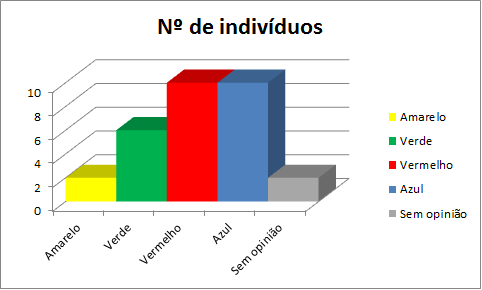
\includegraphics[scale=0.8]{grafico7.jpg}  

\legend{Fonte: www.Google.com.br}
\end{center}
\end{figure}

\subsubsection{Polígono de Frequência}

Um polígono de frequência é um gráfico que se realiza através da união dos pontos mais altos das
colunas num histograma de frequência. Eles são feitos a partir da marca de classe que coincide com o ponto médio de cada coluna do histograma (meio de cada amplitude de classe). Quando são representadas as
frequências acumuladas de uma tabela de dados agrupados, obtém-se um histograma de frequências
acumuladas, que permite dispor em diagrama o seu polígono correspondente.\cite{poligono}

Geralmente, os polígonos de frequência são usados quando se pretende mostrar mais de uma
distribuição ou a classificação cruzada de uma variável quantitativa contínua com uma qualitativa ou
quantitativa discreta num mesmo gráfico. O ponto que tiver mais altura num polígono de frequência representa a maior frequência, ao passo que a área abaixo da curva inclui a totalidade dos dados existentes. 

\textbf{Exemplo:}

Considerando as idades de 50 funcionários de uma empresa, agrupados conforme a tabela a seguir:

\begin{center}
\begin{table}[H]
\caption{Tabela das idades dos funcionários}
\begin{center}
\begin{tabular}{c|c|c}

\hline
Classes & Intervalos & Frequência $(\%)$ \\ 
\hline
1 & 18$\vdash$ 25 & 6 \\
\hline
2 & 25$\vdash$ 32 & 10 \\
\hline
3 & 32$\vdash$ 39 & 13 \\
\hline
4 & 39$\vdash$ 46 & 8 \\
\hline
5 & 46$\vdash$ 53 & 6 \\
\hline
6 & 53$\vdash$ 60 & 5 \\
\hline
7 & 60$\vdash$ 66 & 2 \\
\hline
Total &  & 50 \\

\end{tabular}
\end{center}
\legend{Fonte: www.professorguru.com.br}
\end{table}
\end{center}

\begin{figure}[H]
\begin{center}

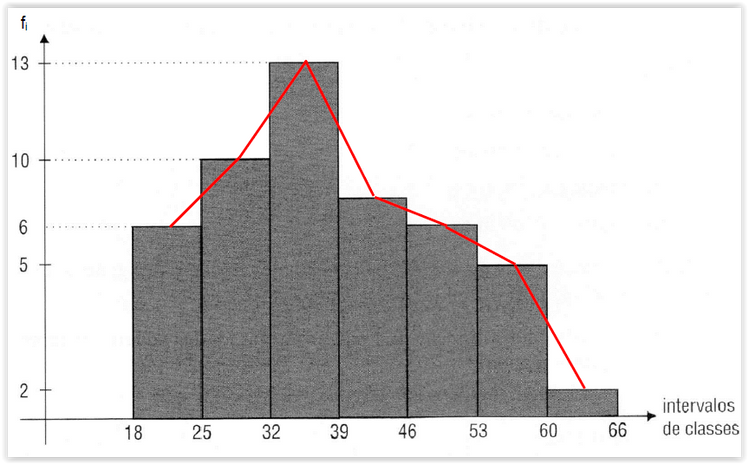
\includegraphics[scale=0.5]{grafico6.jpg}  

\legend{Fonte: www.professorguru.com.br}
\end{center}
\end{figure}

\subsubsection{BoxPlot}

O gráfico BoxPlot é o mais completo dentre todos, pois, em seu ambiente conseguimos notar muitos dados que o histograma não apresenta. Entre esses dados notamos: 1º e 3º quartil, a mediana e os limites inferiores e superiores (esses dois últimos, no entanto, são apresentados no histograma também).

O boxplot tem uma reta (whisker) que estende–se verticalmente ou horizontalmente a partir da caixa, indicando a variabilidade fora do quartil superior e do quartil inferior. Os valores atípicos ou outliers podem ser plotados como pontos individuais. Os espaços entre as diferentes partes da caixa indicam o grau de dispersão, a obliquidade nos dados e os outliers.\cite{wiki}

\textbf{Exemplo:} 

Uma indústria produz uma peça automotiva cujo valor de referência é 75cm. Após verificar peças fora dos padrões, enviaram duas equipes de trabalhadores (A e B) para um treinamento. Para verificar a eficiência do treinamento, foram selecionadas 10 peças produzidas pelas equipes A e B e 10 peças produzidas pelas equipes C e D que não participaram do treinamento.

\begin{center}
\begin{table}[H]
\caption{Tamanho das peças produzidas pelas 4 equipes}
\begin{center}
\begin{tabular}{c|c|c|c}

\hline
Equipe A & Equipe B & Equipe C & Equipe D $(\%)$ \\ 
\hline
75,27 & 74,94 & 75,93 & 75,98 \\
\hline
75,33 & 75,25 & 76,95 & 75,61 \\
\hline
74,58 & 75,44 & 75,47 & 74,20 \\
\hline
75,01 & 74,62 & 73,60 & 76,44 \\
\hline
75,71 & 75,35 & 74,85 & 76,84 \\
\hline
74,93 & 74,75 & 73,34 & 76,75 \\
\hline
74,72 & 74,65 & 74,04 & 76,78 \\
\hline
74,53 & 74,94 & 75,00 & 74,74 \\
\hline
75,32 & 74,92 & 76,18 & 72,58 \\
\hline
74,05 & 75,46 & 75,33 & 72,86 \\

\end{tabular}
\end{center}
\legend{Fonte: www.portalaction.com.br}
\end{table}
\end{center}

\begin{figure}[H]
\begin{center}

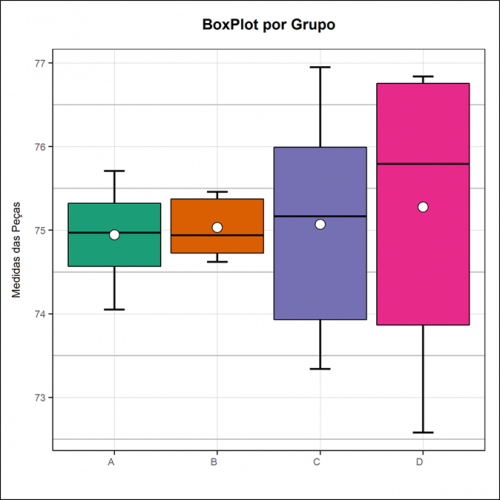
\includegraphics[scale=0.55]{grafico5.jpg}  

\legend{Fonte: www.portalaction.com.br}
\end{center}
\end{figure}

% ---
% inserir lista de ilustrações
% ---
%\pdfbookmark[0]{\listfigurename}{lof}
%\listoffigures*
%\cleardoublepage
% ---

% ---
% inserir lista de tabelas
% ---
%\pdfbookmark[0]{\listtablename}{lot}
%\listoftables*
%\cleardoublepage
% ---

% ---
% inserir lista de abreviaturas e siglas
% ---
%\begin{siglas}
% \item[ABNT] Associação Brasileira de Normas Técnicas
%  \item[abnTeX] ABsurdas Normas para TeX
%\end{siglas}
% ---

% ---
% inserir lista de símbolos
% ---
%\begin{simbolos}
  %\item[$ \Gamma $] Letra grega Gama
  %\item[$ \Lambda $] Lambda
  %\item[$ \zeta $] Letra grega minúscula zeta
  %\item[$ \in $] Pertence
%\end{simbolos}
% ---

% ----------------------------------------------------------
% ELEMENTOS TEXTUAIS
% ----------------------------------------------------------
\newpage
\section[Conclusão]{Conclusão}
\pagestyle{fancy}

Estatística é uma ciência exata que visa fornecer subsídios ao analista para coletar, organizar, resumir, analisar e apresentar dados.\cite{mat} Para que esses dados sejam de fácil entendimento e visualização foram criadas: Tabelas de frequência e diferentes tipos de gráficos. E tudo isso dividido conforme o tipo de variável com a qual se está trabalhando seja ela qualitativa, nominal ou ordinal, ou quantitativa, discreta ou contínua.

Tal ciência é importante método de gestão nos dias atuais, e é utilizada na maioria das vezes para aumentar a credibilidade de argumentos, pois, nada mais são que pesquisas feitas para entendermos como uma amostra ou população está sendo afetada.\cite{conc1}

Estatística é método, ciência e arte. É método quando, na Física, na Biologia, na Medicina ou na Pedagogia, aplica-se a populações específicas, isto é, serve a uma ciência particular, da qual se torna instrumento. É ciência quando, graças às suas teorias, estuda grandes conjuntos, independentemente da natureza destes, sendo autônoma e universal. Finalmente, é arte na construção de modelos para representar a realidade.\cite{conc}


% ----------------------------------------------------------
% Glossário
% ----------------------------------------------------------
%
% Consulte o manual da classe abntex2 para orientações sobre o glossário.
%
%\glossary

\bibliographystyle{ieeetr}
\bibliography{Ref}

\end{document}
